\documentclass[a4paper,10pt]{article}

\usepackage{amsmath}
\usepackage{float}
\usepackage{graphicx}
\usepackage{tikz,ifthen}
\usetikzlibrary{calc}
\usepackage[toc, acronym]{glossaries}
\usepackage{hyperref}
\usepackage[toc, acronym]{glossaries}

\hypersetup{colorlinks=true, linkcolor=black}

\newacronym{lgca}{LGCA}{Lattice-Gas Cellular Automata}
\newacronym{lbm}{LBM}{lattice Boltzmann models}
\newtheorem{theorem}{Theorem}[section]
\newtheorem{lemma}[theorem]{Lemma}
\newtheorem{proposition}[theorem]{Proposition}
\newtheorem{corollary}[theorem]{Corollary}
\newenvironment{definition}[1][Definition]{\begin{trivlist}
\item[\hskip \labelsep {\bfseries #1}]}{\end{trivlist}}

\author{Mr. S. Schreiber}
\date{\today}
\title{Flow modelling with lattice gas cellular automata}
%glossary entries
\newglossaryentry{EP}
{
	name = {pauli exclusion principle},
	description={is the quantum mechanical principle that no 			two identical fermions may occupy the same quantum state 			simultaneously.}
}


\begin{document}
\maketitle
\begin{abstract}
The use of lattice in flow modelling has become increasingly popular over the last couple of decades and during that time a lot of models have been developed. We'll be investigating three of the more widely used models i.e. FHP and \acrshort{lbm}. The following will be discussed for each model: history, assumptions, the collision rules, the propagation rules, calculation of the mass and momentum density, time complexity analysis, applications, defects and does it obey the desired hydrodynamics equation (Navier Stokes) in the macroscopic limit. 
\end{abstract}
\section{Introduction}

\section{Background}
\subsection{Cellular automata}
Informally a cellular automaton is a system made up of many discrete cells, usually a M by N grid. Each one of these cells can be in one of a finite number of states. Each cell or automaton may only change state on a fixed interval and only according to a fixed set of rules. These rules depend on the cells own value and that of this neighbours. A cellular automaton can formally be defined by
\begin{definition}
A cellular automaton is a 4-tuple, $C = \{S,s_{0},f,G\}$, where
\begin{enumerate}
\item $S$ is a finite set of state,
\item $s_{0}$ is the initial state,
\item $G$ is the neighbourhood,
\item $f:S^{n} \rightarrow S$.
\end{enumerate}
\end{definition}
Two popular neighbourhoods are the von Neumann and Moore.
The von Neumann neighbourhood for range r can be defined by \[ G_{(x_{0}, y_{0})} = \{(x, y): \left|x - x_{0} \right| + \left|y - y_{0}\right| \leq r\}.\]
The Moore neighbourhood for range r can be defined by \[ G_{(x_{0}, y_{0})} = \{(x, y): \left|x - x_{0}\right| \leq r, \left|y - y_{0}\right| \leq r \}.\]
A popular example of a cellular automata that makes use of a Moore neighbourhood with r = 1 is ``Conway's game of life''.
\subsection{Lattice gas cellular automata}
Lattice gas cellular automata is a cellular automata where the transition functions $f$ is split into two phases i.e. propagation phase and collision phase. Also each cell has n number of local sites, where n is the number of directly connected neighbours. Each site is associated with a specific velocity vector $\textbf{c}_{i}$ $( i = 0,1,2,\dots,n)$. Velocity vectors are the edge's between cells and their neighbours and is of unit length. Sites may be empty or occupied by at most one particle. This \gls{EP} is characteristic for all lattice-gas cellular automata.   
\begin{figure}[H]
  \centering
  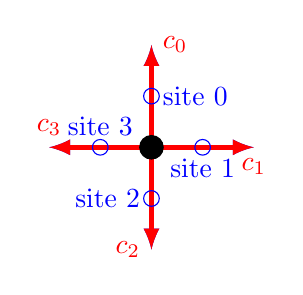
\begin{tikzpicture}[scale=0.65]

    \coordinate (Origin) at (0,0);
    \coordinate (site1) at (0,2);
    \coordinate (site2) at (2,0);
    \coordinate (site3) at (0,-2);
    \coordinate (site4) at (-2,0);  
    
    \draw [ultra thick,-latex,blue] (Origin)
        -- (site1) node [midway, right] {site 0};
    \draw [ultra thick,-latex,blue] (Origin)
        -- (site2) node [midway,below] {site 1};
    \draw [ultra thick,-latex,blue] (Origin)
        -- (site3) node [midway,left] {site 2};
    \draw [ultra thick,-latex,blue] (Origin)
        -- (site4) node [midway,above] {site 3};
        
	\draw [ultra thick,-latex,red] (Origin)
        -- (site1) node [right] {$c_0$};
    \draw [ultra thick,-latex,red] (Origin)
        -- (site2) node [below] {$c_1$};
    \draw [ultra thick,-latex,red] (Origin)
        -- (site3) node [left] {$c_2$};
    \draw [ultra thick,-latex,red] (Origin)
        -- (site4) node [above] {$c_3$};
       
    \node[draw,circle,inner sep=3pt,fill] at (0,0) {};
    \node[draw,circle,inner sep=2pt,blue] at (1,0) {};
	\node[draw,circle,inner sep=2pt,blue] at (0,1) {};
	\node[draw,circle,inner sep=2pt,blue] at (-1,0) {};
	\node[draw,circle,inner sep=2pt,blue] at (0,-1) {};
  \end{tikzpicture}
  \caption{Here is an example of a single cell with 4 velocity vectors and 4 empty sites.}
  \label{figure:single-cell}
\end{figure}
\noindent As previously mentioned the transition function $f$ is divided into two phases propagation and collision.
The collision phase only applies rules that act on a single cell i.e. the local sites.
The propagation phase on the other hand applies rules between cells. What those rules are will vary between implementations and will be discussed later.

\section{\acrfull{lgca}}
\subsection{HPP}
\subsubsection{History}
The HPP model was proposed by Hardy, de Pazzis and Pomeau in 1973.
This was the first \acrshort{lgca} model and received its name from the initials of the authors. It is the simplest \acrshort{lgca} model and is only mentioned for its historical importance and not for its application because it does not lead to the Navier-Stokes equation in the macroscopic limit, this is due to the insufficient degree of rotational symmetry of the lattice. 
\subsubsection{Model Description}
The HPP model is a \acrshort{lgca} that make use of a square lattice.
Each cell has 4 velocity vectors $\textbf{c}_{i}$ where $i \in \{0, 1, 2, 3\}$. Each velocity vector is associated with one site, see Fig \ref{figure:single-cell}. All particles have the same mass m and are indistinguishable. A site can only be in one of two states occupied or empty. A site can not be occupied by more than one particle (\Gls{EP}). It will lead to equilibrium distributions of Fermi-Dirac type for
the mean occupation of the cells.%Cite this
The two phase will now be discussed.
\subsubsection{Collision phase}
This is a basic model and thus only has one collision rule, all other configurations are treated as if no collisions have occurred. The collision rules only consider local sites and only has a local effect. The notation to select the nth site is $s_{n}$. If $s_{i}$ is equals to the opposite site $s_{j}$ where $j = (i + 2)\bmod{4}$ and the other two sites are empty. Then $s_{k}$ will take the value of $s_{i}$ and $s_{d}$ will take the value of $s_{j}$ where k and d are the indices of the open sites. The sites $s_{j}$ and $s_{i}$ are then set to empty.
\begin{figure}[H]
\begin{minipage}[width=0.5\linewidth]{0.5\textwidth}
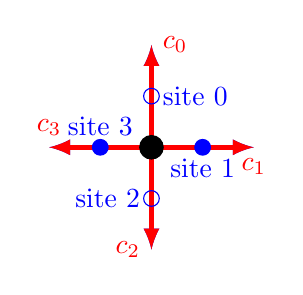
\begin{tikzpicture}[scale=0.65]
    \coordinate (Origin) at (0,0);
    \coordinate (site1) at (0,2);
    \coordinate (site2) at (2,0);
    \coordinate (site3) at (0,-2);
    \coordinate (site4) at (-2,0);  
    
    \draw [ultra thick,-latex,blue] (Origin)
        -- (site1) node [midway, right] {site 0};
    \draw [ultra thick,-latex,blue] (Origin)
        -- (site2) node [midway,below] {site 1};
    \draw [ultra thick,-latex,blue] (Origin)
        -- (site3) node [midway,left] {site 2};
    \draw [ultra thick,-latex,blue] (Origin)
        -- (site4) node [midway,above] {site 3};
        
	\draw [ultra thick,-latex,red] (Origin)
        -- (site1) node [right] {$c_0$};
    \draw [ultra thick,-latex,red] (Origin)
        -- (site2) node [below] {$c_1$};
    \draw [ultra thick,-latex,red] (Origin)
        -- (site3) node [left] {$c_2$};
    \draw [ultra thick,-latex,red] (Origin)
        -- (site4) node [above] {$c_3$};
       
    \node[draw,circle,inner sep=3pt,fill] at (0,0) {};
    \node[draw,circle,inner sep=2pt,fill,blue] at (1,0) {};
	\node[draw,circle,inner sep=2pt,blue] at (0,1) {};
	\node[draw,circle,inner sep=2pt,fill,blue] at (-1,0) {};
	\node[draw,circle,inner sep=2pt,blue] at (0,-1) {};
  \end{tikzpicture}
  \caption{Before Collision}
  \label{figure:collision_HPP1}
\end{minipage} 
\begin{minipage}[width=0.5\linewidth]{0.5\textwidth}
 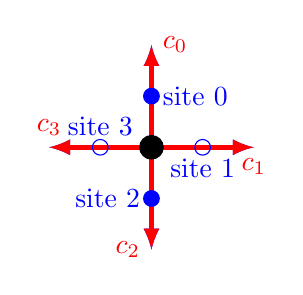
\begin{tikzpicture}[scale=0.65]
    \coordinate (Origin) at (0,0);
    \coordinate (site1) at (0,2);
    \coordinate (site2) at (2,0);
    \coordinate (site3) at (0,-2);
    \coordinate (site4) at (-2,0);  
    
    \draw [ultra thick,-latex,blue] (Origin)
        -- (site1) node [midway, right] {site 0};
    \draw [ultra thick,-latex,blue] (Origin)
        -- (site2) node [midway,below] {site 1};
    \draw [ultra thick,-latex,blue] (Origin)
        -- (site3) node [midway,left] {site 2};
    \draw [ultra thick,-latex,blue] (Origin)
        -- (site4) node [midway,above] {site 3};
        
	\draw [ultra thick,-latex,red] (Origin)
        -- (site1) node [right] {$c_0$};
    \draw [ultra thick,-latex,red] (Origin)
        -- (site2) node [below] {$c_1$};
    \draw [ultra thick,-latex,red] (Origin)
        -- (site3) node [left] {$c_2$};
    \draw [ultra thick,-latex,red] (Origin)
        -- (site4) node [above] {$c_3$};
       
    \node[draw,circle,inner sep=3pt,fill] at (0,0) {};
    \node[draw,circle,inner sep=2pt,blue] at (1,0) {};
	\node[draw,circle,inner sep=2pt,fill,blue] at (0,1) {};
	\node[draw,circle,inner sep=2pt,blue] at (-1,0) {};
	\node[draw,circle,inner sep=2pt,fill,blue] at (0,-1) {};
  \end{tikzpicture}
  \caption{After Collision}
  \label{figure:collision_HPP2}
\end{minipage} 
\end{figure}
\subsubsection{Propagation phase}
The propagation phase only considers the local neighbours of a cell and not the cell it self. The propagation phase has no effect on the local neighbours of a cell, only on the cell it self. The cell's neighbours will be denoted as $n_i$ where $i \in \{0, 1, 2, 3\}$, the cell it self does not count as a neighbour. Neighbour $n_0$ is the top neighbour, neighbour $n_1$ is tot the right, neighbour $n_2$ is below and neighbour $n_3$ is tot the left of the cell. The propagation rules work as follow: If the cell's neighbour $n_i$ has a occupied site $s_{i}$ then the particle in that site moves to the cell's
site $s_{i}$.
A thing to keep in mind while applying the propagation phase is, that it will require two states/matrices one that stores the previous results and one that will store the new results.

\begin{figure}[H]
\begin{minipage}{0.33\textwidth}
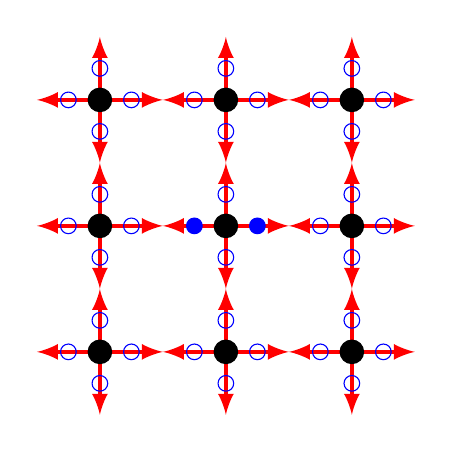
\begin{tikzpicture}[scale=0.4]
\foreach \x in {-4, 0, 4}
	{
	\foreach \y in {-4, 0, 4}
		{
		\ifthenelse{\x = 0 \AND \y = 0}{
    		\coordinate (Origin) at (0 + \x, 0 + \y);
    		\coordinate (site1) at (0+ \x,2+ \y);
    		\coordinate (site2) at (2+ \x,0+ \y);
    		\coordinate (site3) at (0+ \x,-2+ \y);
    		\coordinate (site4) at (-2+ \x,0+ \y);  
    
 
        
		\draw [ultra thick,-latex,red] (Origin)
   		     -- (site1) node [right] {};
    		\draw [ultra thick,-latex,red] (Origin)
        		-- (site2) node [below] {};
    		\draw [ultra thick,-latex,red] (Origin)
        		-- (site3) node [left] {};
    		\draw [ultra thick,-latex,red] (Origin)
        		-- (site4) node [above] {};
       
    		\node[draw,circle,inner sep=3pt,fill] at (0+ \x,0+ \y) {};
    		\node[draw,circle,inner sep=2pt,fill,blue] at (1+ \x,0+ \y) {};
		\node[draw,circle,inner sep=2pt,blue] at (0+ \x,1+ \y) {};
		\node[draw,circle,inner sep=2pt,fill,blue] at (-1+ \x,0+ \y) {};
		\node[draw,circle,inner sep=2pt,blue] at (0+ \x,-1+ \y) {};
		}%else
		{
		
    		\coordinate (Origin) at (0 + \x, 0 + \y);
    		\coordinate (site1) at (0+ \x,2+ \y);
    		\coordinate (site2) at (2+ \x,0+ \y);
    		\coordinate (site3) at (0+ \x,-2+ \y);
    		\coordinate (site4) at (-2+ \x,0+ \y);  
    

        
		\draw [ultra thick,-latex,red] (Origin)
   		     -- (site1) node [right] {};
    		\draw [ultra thick,-latex,red] (Origin)
        		-- (site2) node [below] {};
    		\draw [ultra thick,-latex,red] (Origin)
        		-- (site3) node [left] {};
    		\draw [ultra thick,-latex,red] (Origin)
        		-- (site4) node [above] {};
       
    		\node[draw,circle,inner sep=3pt,fill] at (0+ \x,0+ \y) {};
    		\node[draw,circle,inner sep=2pt,blue] at (1+ \x,0+ \y) {};
		\node[draw,circle,inner sep=2pt,blue] at (0+ \x,1+ \y) {};
		\node[draw,circle,inner sep=2pt,blue] at (-1+ \x,0+ \y) {};
		\node[draw,circle,inner sep=2pt,blue] at (0+ \x,-1+ \y) {};
		}
		}
	}
  \end{tikzpicture}
   
  \caption{Initial configuration, before collision}
  \label{figure:collision_HPP3} 
   \end{minipage}
\begin{minipage}{0.33\textwidth}
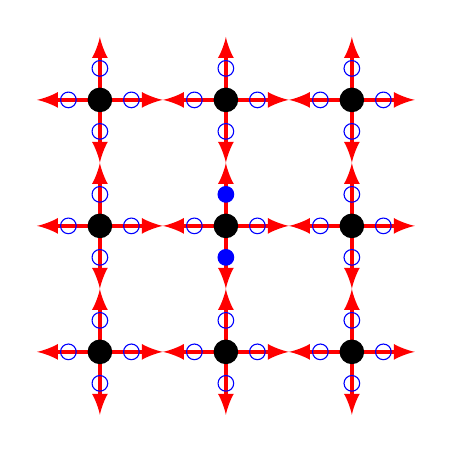
\begin{tikzpicture}[scale=0.4]
\foreach \x in {-4, 0, 4}
	{
	\foreach \y in {-4, 0, 4}
		{
		\ifthenelse{\x = 0 \AND \y = 0}{
    		\coordinate (Origin) at (0 + \x, 0 + \y);
    		\coordinate (site1) at (0+ \x,2+ \y);
    		\coordinate (site2) at (2+ \x,0+ \y);
    		\coordinate (site3) at (0+ \x,-2+ \y);
    		\coordinate (site4) at (-2+ \x,0+ \y);  
        
		\draw [ultra thick,-latex,red] (Origin)
   		     -- (site1) node [right] {};
    		\draw [ultra thick,-latex,red] (Origin)
        		-- (site2) node [below] {};
    		\draw [ultra thick,-latex,red] (Origin)
        		-- (site3) node [left] {};
    		\draw [ultra thick,-latex,red] (Origin)
        		-- (site4) node [above] {};
       
    		\node[draw,circle,inner sep=3pt,fill] at (0+ \x,0+ \y) {};
    		\node[draw,circle,inner sep=2pt,blue] at (1+ \x,0+ \y) {};
		\node[draw,circle,inner sep=2pt,fill,blue] at (0+ \x,1+ \y) {};
		\node[draw,circle,inner sep=2pt,blue] at (-1+ \x,0+ \y) {};
		\node[draw,circle,inner sep=2pt,fill,blue] at (0+ \x,-1+ \y) {};
		}%else
		{
		
    		\coordinate (Origin) at (0 + \x, 0 + \y);
    		\coordinate (site1) at (0+ \x,2+ \y);
    		\coordinate (site2) at (2+ \x,0+ \y);
    		\coordinate (site3) at (0+ \x,-2+ \y);
    		\coordinate (site4) at (-2+ \x,0+ \y);  
        
		\draw [ultra thick,-latex,red] (Origin)
   		     -- (site1) node [right] {};
    		\draw [ultra thick,-latex,red] (Origin)
        		-- (site2) node [below] {};
    		\draw [ultra thick,-latex,red] (Origin)
        		-- (site3) node [left] {};
    		\draw [ultra thick,-latex,red] (Origin)
        		-- (site4) node [above] {};
       
    		\node[draw,circle,inner sep=3pt,fill] at (0+ \x,0+ \y) {};
    		\node[draw,circle,inner sep=2pt,blue] at (1+ \x,0+ \y) {};
		\node[draw,circle,inner sep=2pt,blue] at (0+ \x,1+ \y) {};
		\node[draw,circle,inner sep=2pt,blue] at (-1+ \x,0+ \y) {};
		\node[draw,circle,inner sep=2pt,blue] at (0+ \x,-1+ \y) {};
		}
		}
	}
  \end{tikzpicture}
  \caption{After Collision and before propagation}
  \label{figure:propagation_HPP1} 
   \end{minipage}
   \begin{minipage}{0.33\textwidth}
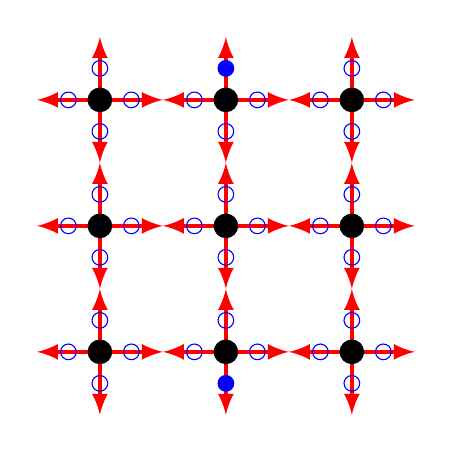
\begin{tikzpicture}[scale=0.4]
\foreach \x in {-4, 0, 4}
	{
	\foreach \y in {-4, 0, 4}
		{
		\ifthenelse{\x = 0 \AND \y = -4}{
    			\coordinate (Origin) at (0 + \x, 0 + \y);
    			\coordinate (site1) at (0+ \x,2+ \y);
    			\coordinate (site2) at (2+ \x,0+ \y);
    			\coordinate (site3) at (0+ \x,-2+ \y);
    			\coordinate (site4) at (-2+ \x,0+ \y);  
        
			\draw [ultra thick,-latex,red] (Origin)
   			     -- (site1) node [right] {};
    			\draw [ultra thick,-latex,red] (Origin)
        			-- (site2) node [below] {};
    			\draw [ultra thick,-latex,red] (Origin)
        			-- (site3) node [left] {};
    			\draw [ultra thick,-latex,red] (Origin)
        			-- (site4) node [above] {};
       
    			\node[draw,circle,inner sep=3pt,fill] at (0+ \x,0+ \y) {};
    			\node[draw,circle,inner sep=2pt,blue] at (1+ \x,0+ \y) {};
			\node[draw,circle,inner sep=2pt,blue] at (0+ \x,1+ \y) {};
			\node[draw,circle,inner sep=2pt,blue] at (-1+ \x,0+ \y) {};
			\node[draw,circle,inner sep=2pt,fill,blue] at (0+ \x,-1+ \y) {};
		}%else
		{
			\ifthenelse{\x = 0 \AND \y = 4}
				{
    					\coordinate (Origin) at (0 + \x, 0 + \y);
    					\coordinate (site1) at (0+ \x,2+ \y);
    					\coordinate (site2) at (2+ \x,0+ \y);
    					\coordinate (site3) at (0+ \x,-2+ \y);
    					\coordinate (site4) at (-2+ \x,0+ \y);  
        
					\draw [ultra thick,-latex,red] (Origin)
   					     -- (site1) node [right] {};
    					\draw [ultra thick,-latex,red] (Origin)
       	 				-- (site2) node [below] {};
    					\draw [ultra thick,-latex,red] (Origin)
       	 				-- (site3) node [left] {};
    					\draw [ultra thick,-latex,red] (Origin)
        					-- (site4) node [above] {};
       
    					\node[draw,circle,inner sep=3pt,fill] at (0+ \x,0+ \y) {};
    					\node[draw,circle,inner sep=2pt,blue] at (1+ \x,0+ \y) {};
					\node[draw,circle,inner sep=2pt,fill,blue] at (0+ \x,1+ \y) {};
					\node[draw,circle,inner sep=2pt,blue] at (-1+ \x,0+ \y) {};
					\node[draw,circle,inner sep=2pt,blue] at (0+ \x,-1+ \y) {};
				}% else
				{
					\coordinate (Origin) at (0 + \x, 0 + \y);
    					\coordinate (site1) at (0+ \x,2+ \y);
    					\coordinate (site2) at (2+ \x,0+ \y);
    					\coordinate (site3) at (0+ \x,-2+ \y);
    					\coordinate (site4) at (-2+ \x,0+ \y);  
        
					\draw [ultra thick,-latex,red] (Origin)
   					     -- (site1) node [right] {};
    					\draw [ultra thick,-latex,red] (Origin)
       	 				-- (site2) node [below] {};
    					\draw [ultra thick,-latex,red] (Origin)
       	 				-- (site3) node [left] {};
    					\draw [ultra thick,-latex,red] (Origin)
        					-- (site4) node [above] {};
       
    					\node[draw,circle,inner sep=3pt,fill] at (0+ \x,0+ \y) {};
    					\node[draw,circle,inner sep=2pt,blue] at (1+ \x,0+ \y) {};
					\node[draw,circle,inner sep=2pt,blue] at (0+ \x,1+ \y) {};
					\node[draw,circle,inner sep=2pt,blue] at (-1+ \x,0+ \y) {};
					\node[draw,circle,inner sep=2pt,blue] at (0+ \x,-1+ \y) {};
				}
			}
		}
	}
  \end{tikzpicture}
  \caption{After propagation}
  \label{figure:propagation_HPP2} 
   \end{minipage}
\end{figure}
\subsubsection{Boundary conditions}
We will discuss two approaches to handle the boundary condition i.e. wrap around (also known as repeating) and reflection. Both conditions only have an effect on the propagation phase and not on the collision phase. Also when generating a lattice grid and using the reflection boundary condition do not generate particles in the border sites\footnote{Border sites are the sites right next to the border and not all 4 sites of the border cell} this will create problems.
\paragraph{Wrap around}
This approach can easily be explained by firstly placing copies of the current lattice all around it self i.e all 4 positions. The center lattice is the original while the other 4 lattices are copies.
Secondly by running the propagation phase on the new lattice. All the changes that happen in the center lattice must then be applied to the original\footnote{What is meant by original lattice is the lattice that was created after the collision phase has executed} lattice. All of the changes that happen in copies are ignored. This effect can also easily be achieved by making use of the module operator.
\begin{figure}[H]
\begin{minipage}{0.5\textwidth}
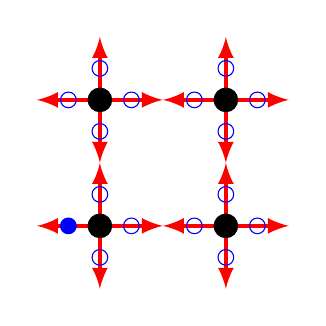
\begin{tikzpicture}[scale=0.4]
\foreach \x in {0, 4}
	{
	\foreach \y in {0, 4}
		{
		\ifthenelse{\x = 0 \AND \y = 0}{
    		\coordinate (Origin) at (0 + \x, 0 + \y);
    		\coordinate (site1) at (0+ \x,2+ \y);
    		\coordinate (site2) at (2+ \x,0+ \y);
    		\coordinate (site3) at (0+ \x,-2+ \y);
    		\coordinate (site4) at (-2+ \x,0+ \y);  
    
 
        
		\draw [ultra thick,-latex,red] (Origin)
   		     -- (site1) node [right] {};
    		\draw [ultra thick,-latex,red] (Origin)
        		-- (site2) node [below] {};
    		\draw [ultra thick,-latex,red] (Origin)
        		-- (site3) node [left] {};
    		\draw [ultra thick,-latex,red] (Origin)
        		-- (site4) node [above] {};
       
    		\node[draw,circle,inner sep=3pt,fill] at (0+ \x,0+ \y) {};
    		\node[draw,circle,inner sep=2pt,blue] at (1+ \x,0+ \y) {};
		\node[draw,circle,inner sep=2pt,blue] at (0+ \x,1+ \y) {};
		\node[draw,circle,inner sep=2pt,fill,blue] at (-1+ \x,0+ \y) {};
		\node[draw,circle,inner sep=2pt,blue] at (0+ \x,-1+ \y) {};
		}%else
		{
		
    		\coordinate (Origin) at (0 + \x, 0 + \y);
    		\coordinate (site1) at (0+ \x,2+ \y);
    		\coordinate (site2) at (2+ \x,0+ \y);
    		\coordinate (site3) at (0+ \x,-2+ \y);
    		\coordinate (site4) at (-2+ \x,0+ \y);  
    

        
		\draw [ultra thick,-latex,red] (Origin)
   		     -- (site1) node [right] {};
    		\draw [ultra thick,-latex,red] (Origin)
        		-- (site2) node [below] {};
    		\draw [ultra thick,-latex,red] (Origin)
        		-- (site3) node [left] {};
    		\draw [ultra thick,-latex,red] (Origin)
        		-- (site4) node [above] {};
       
    		\node[draw,circle,inner sep=3pt,fill] at (0+ \x,0+ \y) {};
    		\node[draw,circle,inner sep=2pt,blue] at (1+ \x,0+ \y) {};
		\node[draw,circle,inner sep=2pt,blue] at (0+ \x,1+ \y) {};
		\node[draw,circle,inner sep=2pt,blue] at (-1+ \x,0+ \y) {};
		\node[draw,circle,inner sep=2pt,blue] at (0+ \x,-1+ \y) {};
		}
		}
	}
  \end{tikzpicture}
   
  \caption{Initial configuration}
  \label{figure:boundary_HPP1} 
   \end{minipage}
   \begin{minipage}{0.5\textwidth}
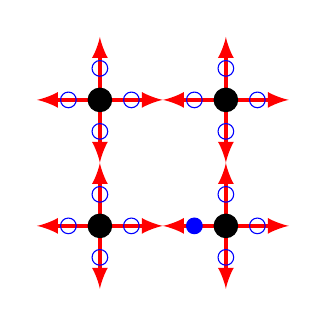
\begin{tikzpicture}[scale=0.4]
\foreach \x in {0, 4}
	{
	\foreach \y in {0, 4}
		{
		\ifthenelse{\x = 4 \AND \y = 0}{
    		\coordinate (Origin) at (0 + \x, 0 + \y);
    		\coordinate (site1) at (0+ \x,2+ \y);
    		\coordinate (site2) at (2+ \x,0+ \y);
    		\coordinate (site3) at (0+ \x,-2+ \y);
    		\coordinate (site4) at (-2+ \x,0+ \y);  
    
 
        
		\draw [ultra thick,-latex,red] (Origin)
   		     -- (site1) node [right] {};
    		\draw [ultra thick,-latex,red] (Origin)
        		-- (site2) node [below] {};
    		\draw [ultra thick,-latex,red] (Origin)
        		-- (site3) node [left] {};
    		\draw [ultra thick,-latex,red] (Origin)
        		-- (site4) node [above] {};
       
    		\node[draw,circle,inner sep=3pt,fill] at (0+ \x,0+ \y) {};
    		\node[draw,circle,inner sep=2pt,blue] at (1+ \x,0+ \y) {};
		\node[draw,circle,inner sep=2pt,blue] at (0+ \x,1+ \y) {};
		\node[draw,circle,inner sep=2pt,fill,blue] at (-1+ \x,0+ \y) {};
		\node[draw,circle,inner sep=2pt,blue] at (0+ \x,-1+ \y) {};
		}%else
		{
		
    		\coordinate (Origin) at (0 + \x, 0 + \y);
    		\coordinate (site1) at (0+ \x,2+ \y);
    		\coordinate (site2) at (2+ \x,0+ \y);
    		\coordinate (site3) at (0+ \x,-2+ \y);
    		\coordinate (site4) at (-2+ \x,0+ \y);  
    

        
		\draw [ultra thick,-latex,red] (Origin)
   		     -- (site1) node [right] {};
    		\draw [ultra thick,-latex,red] (Origin)
        		-- (site2) node [below] {};
    		\draw [ultra thick,-latex,red] (Origin)
        		-- (site3) node [left] {};
    		\draw [ultra thick,-latex,red] (Origin)
        		-- (site4) node [above] {};
       
    		\node[draw,circle,inner sep=3pt,fill] at (0+ \x,0+ \y) {};
    		\node[draw,circle,inner sep=2pt,blue] at (1+ \x,0+ \y) {};
		\node[draw,circle,inner sep=2pt,blue] at (0+ \x,1+ \y) {};
		\node[draw,circle,inner sep=2pt,blue] at (-1+ \x,0+ \y) {};
		\node[draw,circle,inner sep=2pt,blue] at (0+ \x,-1+ \y) {};
		}
		}
	}
  \end{tikzpicture}
   
  \caption{After propagation with repeating boundary condition.}
  \label{figure:boundary_HPP2} 
   \end{minipage}
\end{figure}
\paragraph{Reflection} 
This is a easy and quick approach to handle the boundary conditions.
When a particle collides with the boundary it changes its direction by $180^{\circ}$, note by moving a particle to the apposite site is the same as rotating by $180^{\circ}$. It then propagates in that direction.
\begin{figure}[H]
\begin{minipage}{0.29\textwidth}
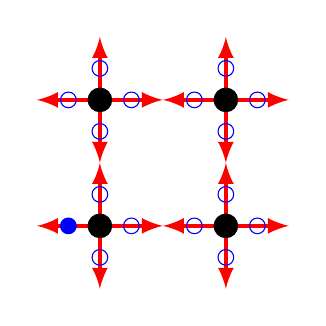
\begin{tikzpicture}[scale=0.4]
\foreach \x in {0, 4}
	{
	\foreach \y in {0, 4}
		{
		\ifthenelse{\x = 0 \AND \y = 0}{
    		\coordinate (Origin) at (0 + \x, 0 + \y);
    		\coordinate (site1) at (0+ \x,2+ \y);
    		\coordinate (site2) at (2+ \x,0+ \y);
    		\coordinate (site3) at (0+ \x,-2+ \y);
    		\coordinate (site4) at (-2+ \x,0+ \y);  
    
 
        
		\draw [ultra thick,-latex,red] (Origin)
   		     -- (site1) node [right] {};
    		\draw [ultra thick,-latex,red] (Origin)
        		-- (site2) node [below] {};
    		\draw [ultra thick,-latex,red] (Origin)
        		-- (site3) node [left] {};
    		\draw [ultra thick,-latex,red] (Origin)
        		-- (site4) node [above] {};
       
    		\node[draw,circle,inner sep=3pt,fill] at (0+ \x,0+ \y) {};
    		\node[draw,circle,inner sep=2pt,blue] at (1+ \x,0+ \y) {};
		\node[draw,circle,inner sep=2pt,blue] at (0+ \x,1+ \y) {};
		\node[draw,circle,inner sep=2pt,fill,blue] at (-1+ \x,0+ \y) {};
		\node[draw,circle,inner sep=2pt,blue] at (0+ \x,-1+ \y) {};
		}%else
		{
		
    		\coordinate (Origin) at (0 + \x, 0 + \y);
    		\coordinate (site1) at (0+ \x,2+ \y);
    		\coordinate (site2) at (2+ \x,0+ \y);
    		\coordinate (site3) at (0+ \x,-2+ \y);
    		\coordinate (site4) at (-2+ \x,0+ \y);  
    

        
		\draw [ultra thick,-latex,red] (Origin)
   		     -- (site1) node [right] {};
    		\draw [ultra thick,-latex,red] (Origin)
        		-- (site2) node [below] {};
    		\draw [ultra thick,-latex,red] (Origin)
        		-- (site3) node [left] {};
    		\draw [ultra thick,-latex,red] (Origin)
        		-- (site4) node [above] {};
       
    		\node[draw,circle,inner sep=3pt,fill] at (0+ \x,0+ \y) {};
    		\node[draw,circle,inner sep=2pt,blue] at (1+ \x,0+ \y) {};
		\node[draw,circle,inner sep=2pt,blue] at (0+ \x,1+ \y) {};
		\node[draw,circle,inner sep=2pt,blue] at (-1+ \x,0+ \y) {};
		\node[draw,circle,inner sep=2pt,blue] at (0+ \x,-1+ \y) {};
		}
		}
	}
  \end{tikzpicture}
   
  \caption{Initial configuration}
  \label{figure:boundary_HPP3} 
   \end{minipage}
   \begin{minipage}{0.29\textwidth}
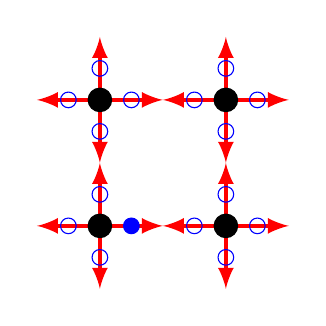
\begin{tikzpicture}[scale=0.4]
\foreach \x in {0, 4}
	{
	\foreach \y in {0, 4}
		{
		\ifthenelse{\x = 0 \AND \y = 0}{
    		\coordinate (Origin) at (0 + \x, 0 + \y);
    		\coordinate (site1) at (0+ \x,2+ \y);
    		\coordinate (site2) at (2+ \x,0+ \y);
    		\coordinate (site3) at (0+ \x,-2+ \y);
    		\coordinate (site4) at (-2+ \x,0+ \y);  
    
 
        
		\draw [ultra thick,-latex,red] (Origin)
   		     -- (site1) node [right] {};
    		\draw [ultra thick,-latex,red] (Origin)
        		-- (site2) node [below] {};
    		\draw [ultra thick,-latex,red] (Origin)
        		-- (site3) node [left] {};
    		\draw [ultra thick,-latex,red] (Origin)
        		-- (site4) node [above] {};
       
    		\node[draw,circle,inner sep=3pt,fill] at (0+ \x,0+ \y) {};
    		\node[draw,circle,inner sep=2pt,fill,blue] at (1+ \x,0+ \y) {};
		\node[draw,circle,inner sep=2pt,blue] at (0+ \x,1+ \y) {};
		\node[draw,circle,inner sep=2pt,blue] at (-1+ \x,0+ \y) {};
		\node[draw,circle,inner sep=2pt,blue] at (0+ \x,-1+ \y) {};
		}%else
		{
		
    		\coordinate (Origin) at (0 + \x, 0 + \y);
    		\coordinate (site1) at (0+ \x,2+ \y);
    		\coordinate (site2) at (2+ \x,0+ \y);
    		\coordinate (site3) at (0+ \x,-2+ \y);
    		\coordinate (site4) at (-2+ \x,0+ \y);  
    

        
		\draw [ultra thick,-latex,red] (Origin)
   		     -- (site1) node [right] {};
    		\draw [ultra thick,-latex,red] (Origin)
        		-- (site2) node [below] {};
    		\draw [ultra thick,-latex,red] (Origin)
        		-- (site3) node [left] {};
    		\draw [ultra thick,-latex,red] (Origin)
        		-- (site4) node [above] {};
       
    		\node[draw,circle,inner sep=3pt,fill] at (0+ \x,0+ \y) {};
    		\node[draw,circle,inner sep=2pt,blue] at (1+ \x,0+ \y) {};
		\node[draw,circle,inner sep=2pt,blue] at (0+ \x,1+ \y) {};
		\node[draw,circle,inner sep=2pt,blue] at (-1+ \x,0+ \y) {};
		\node[draw,circle,inner sep=2pt,blue] at (0+ \x,-1+ \y) {};
		}
		}
	}
  \end{tikzpicture}
   
  \caption{Step one: Turn $180^{\circ}$}
  \label{figure:boundary_HPP4} 
   \end{minipage}
      \begin{minipage}{0.29\textwidth}
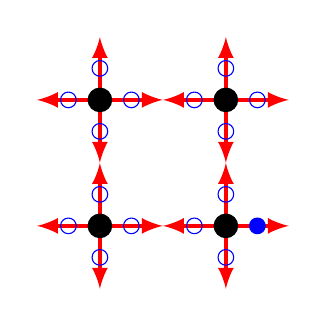
\begin{tikzpicture}[scale=0.4]
\foreach \x in {0, 4}
	{
	\foreach \y in {0, 4}
		{
		\ifthenelse{\x = 4 \AND \y = 0}{
    		\coordinate (Origin) at (0 + \x, 0 + \y);
    		\coordinate (site1) at (0+ \x,2+ \y);
    		\coordinate (site2) at (2+ \x,0+ \y);
    		\coordinate (site3) at (0+ \x,-2+ \y);
    		\coordinate (site4) at (-2+ \x,0+ \y);  
    
 
        
		\draw [ultra thick,-latex,red] (Origin)
   		     -- (site1) node [right] {};
    		\draw [ultra thick,-latex,red] (Origin)
        		-- (site2) node [below] {};
    		\draw [ultra thick,-latex,red] (Origin)
        		-- (site3) node [left] {};
    		\draw [ultra thick,-latex,red] (Origin)
        		-- (site4) node [above] {};
       
    		\node[draw,circle,inner sep=3pt,fill] at (0+ \x,0+ \y) {};
    		\node[draw,circle,inner sep=2pt,fill,blue] at (1+ \x,0+ \y) {};
		\node[draw,circle,inner sep=2pt,blue] at (0+ \x,1+ \y) {};
		\node[draw,circle,inner sep=2pt,blue] at (-1+ \x,0+ \y) {};
		\node[draw,circle,inner sep=2pt,blue] at (0+ \x,-1+ \y) {};
		}%else
		{
		
    		\coordinate (Origin) at (0 + \x, 0 + \y);
    		\coordinate (site1) at (0+ \x,2+ \y);
    		\coordinate (site2) at (2+ \x,0+ \y);
    		\coordinate (site3) at (0+ \x,-2+ \y);
    		\coordinate (site4) at (-2+ \x,0+ \y);  
    

        
		\draw [ultra thick,-latex,red] (Origin)
   		     -- (site1) node [right] {};
    		\draw [ultra thick,-latex,red] (Origin)
        		-- (site2) node [below] {};
    		\draw [ultra thick,-latex,red] (Origin)
        		-- (site3) node [left] {};
    		\draw [ultra thick,-latex,red] (Origin)
        		-- (site4) node [above] {};
       
    		\node[draw,circle,inner sep=3pt,fill] at (0+ \x,0+ \y) {};
    		\node[draw,circle,inner sep=2pt,blue] at (1+ \x,0+ \y) {};
		\node[draw,circle,inner sep=2pt,blue] at (0+ \x,1+ \y) {};
		\node[draw,circle,inner sep=2pt,blue] at (-1+ \x,0+ \y) {};
		\node[draw,circle,inner sep=2pt,blue] at (0+ \x,-1+ \y) {};
		}
		}
	}
  \end{tikzpicture}
   
  \caption{Step 2: Move in that direction.}
  \label{figure:boundary_HPP5} 
   \end{minipage}
\end{figure}
\subsubsection{Mass and Momentum Densities}
The \acrshort{lgca} can be fully describe by the boolean fields $n_{i}(t, \textbf{r}_{j})$, where $i \in \{0, 1, 2, 3\}$, \textbf{r} is the position of the cell and t is the discrete time. $n_{i}(t, \textbf{r}_{j})$ means the boolean value of the ith site at position \textbf{r} at time t.
Before calculating the mass and momentum densities we require the mean occupation numbers. The mean occupation number for site $i$ at position \textbf{x}, is the average of $n_{i}(t, \textbf{r}_{j})$ where 
$\textbf{r}_{j}$ are the the positions of the neighbours of \textbf{x}
\[N_{i}(t,\textbf{x}) = \frac{\sum_{j = 0}^{3} n_{i}(t,\textbf{r}_{j})}{4}.\]
The mass density for time t and position \textbf{x} is defined as follow:
\[\rho(t, \textbf{x}) = \sum_{i = 0}^{3} N_{i}(t, \textbf{x}).\]
The momentum densities for time t and position \textbf{x} is defined as follow:
\[\boldsymbol{j}(t, \textbf{x}) = \rho\boldsymbol{u} = \sum_{i = 0}^{3} \textbf{c}_{i}N_{i}(t, \textbf{x}).\]
\subsubsection{Time complexity analysis}
This is a unoptimized implementation of HHP. It ignores the set-up and boundary costs. Let the lattice size be $n$ by $n$ and the number of occupied sites be l. The collision phase checks each cell to see if a collision has occurred. There are $n^2$ cells and two configurations for each cell. Thus the collision phase has $4n^2$ comparisons.
 The propagation phase checks the 4 neighbours cells to see if any particles will propagate to the current cell which also takes $4n^2$ comparisons. Thus the running time of an unoptimized version of HPP is
 $O(n^2)$.
\subsection{FHP}
\subsubsection{History}
The FHP model was proposed by Frisch, Hasslacher and Pomeau in 1986 and received its name from the initials of the authors. This was the first model that showed it is possible for a \acrshort{lgca} to yield the Navier-Stokes equation in the macroscopic limit. This was a big discovery and lead to the rapid development of lattice-gas cellular automata. There where three FHP models developed FHP-I, FHP-II and FHP-III.
The main difference between each of the models are the collision rules that are used.
\subsubsection{Model Description}
The FHP model is a \acrshort{lgca} that make use of a hexagonal lattice.
Each cell has 6 velocity vectors $\textbf{c}_{i}$ where $i \in \{0, 1, 2, 3, 4, 5\}$ with $60^{\circ}$ between each vector. Also each velocity vector is associated with a site see Fig \ref{figure:Hsingle-cell}. All particles have the same mass m and are indistinguishable. A site can only be in one of two states occupied or empty. A site can not be occupied by more than one particle (\Gls{EP}). It will lead to equilibrium distributions of Fermi-Dirac type for the mean occupation of the cells.%Cite this
\begin{figure}[H]
  \centering
  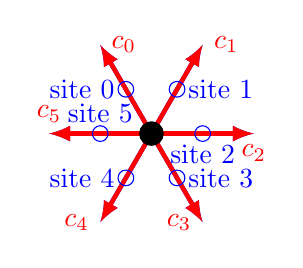
\begin{tikzpicture}[scale=0.65]
  \foreach \x in {0}
	{
	\foreach \y in {0}
		{
    \coordinate (Origin) at (0 + \x,0 + \y);
    \coordinate (site1) at ({2 * cos(120) + \x }, {2 * sin(120) + \y });
    \coordinate (site2) at ({2 * cos(60) + \x }, {2 * sin(60) + \y });
    \coordinate (site3) at ({2 * cos(0) + \x }, {2 * sin(0) + \y });
    \coordinate (site4) at ({2 * cos(-60) + \x }, {2 * sin(-60) + \y });
    \coordinate (site5) at ({2 * cos(-120) + \x }, {2 * sin(-120) + \y });
    \coordinate (site6) at ({2 * cos(-180) + \x }, {2 * sin(-180) + \y });
    
    \draw [ultra thick,-latex,blue] (Origin)
        -- (site1) node [midway, left] {site 0};
    \draw [ultra thick,-latex,blue] (Origin)
        -- (site2) node [midway, right] {site 1};
    \draw [ultra thick,-latex,blue] (Origin)
        -- (site3) node [midway, below] {site 2};
    \draw [ultra thick,-latex,blue] (Origin)
        -- (site4) node [midway, right] {site 3};
    \draw [ultra thick,-latex,blue] (Origin)
        -- (site5) node [midway, left] {site 4};
    \draw [ultra thick,-latex,blue] (Origin)
        -- (site6) node [midway, above] {site 5};     
	\draw [ultra thick,-latex,red] (Origin)
        -- (site1) node [right] {$c_0$};
    \draw [ultra thick,-latex,red] (Origin)
        -- (site2) node [right] {$c_1$};
    \draw [ultra thick,-latex,red] (Origin)
        -- (site3) node [below] {$c_2$};
    \draw [ultra thick,-latex,red] (Origin)
        -- (site4) node [left] {$c_3$};
    \draw [ultra thick,-latex,red] (Origin)
        -- (site5) node [left] {$c_4$};
    \draw [ultra thick,-latex,red] (Origin)
        -- (site6) node [above] {$c_5$};    
 \coordinate (Origin) at (0 + \x,0 + \y);
    \coordinate (site1) at ({cos(120) + \x }, { sin(120) + \y });
    \coordinate (site2) at ({ cos(60) + \x }, { sin(60) + \y });
    \coordinate (site3) at ({ cos(0) + \x }, { sin(0) + \y });
    \coordinate (site4) at ({ cos(-60) + \x }, { sin(-60) + \y });
    \coordinate (site5) at ({ cos(-120) + \x }, { sin(-120) + \y });
    \coordinate (site6) at ({ cos(-180) + \x }, { sin(-180) + \y });
       
    \node[draw,circle,inner sep=3pt,fill] at (Origin) {};
    \node[draw,circle,inner sep=2pt,blue] at (site1) {};
    \node[draw,circle,inner sep=2pt,blue] at (site2) {};
    \node[draw,circle,inner sep=2pt,blue] at (site3) {};
    \node[draw,circle,inner sep=2pt,blue] at (site4) {};
    \node[draw,circle,inner sep=2pt,blue] at (site5) {};
    \node[draw,circle,inner sep=2pt,blue] at (site6) {};
    }
 }
  \end{tikzpicture}
  \caption{Here is an example of a single hexagonal cell with 6 velocity vectors and 6 empty sites.}
  \label{figure:Hsingle-cell}
\end{figure}
\noindent The velocity vectors must have a symmetrical property i.e. $\sum_{i = 0}^{5} \textbf{c}_{i} = \textbf{0}$. Also each vector should be of unit length.
\subsubsection{Collision rules}
The collision rules for FHP are a lot more complex than HPP. FHP also introduced non-determinism in some of the rules because if this was not done the model would become chiral. This is an undesired property because the hydrodynamic equations do not break parity symmetry.
Let $s_{i}$ and $c_{i}$ respectively denote the $i$th site and vector of the current cell where $i \in \{0, 1, 2, 3, 4, 5\}$. 
\paragraph{Rule 1}(2-particle head-on collisions): When two opposite sites are occupied and the rest of the sites are empty,  then a collision has happened. Now are two configurations to choose from. The choice between the two configurations are done randomly with a probability of 0.5. The rule can be defined as: If \[(s_{i} = s_{i + 3})\wedge(s_{i} = 1)\wedge(s_{j} = 0)\wedge(j \neq i)\wedge(j \neq (i + 3)) \mbox{ for } i,j \in \{0, 1, 2, 3, 4, 5\}\] then with p = 0.5 choose \[ (s_{i - 1} := s_{i}), (s_{i + 2} := s_{i + 3})\]or\[(s_{i + 1} := s_{i}), (s_{i + 4} := s_{i + 3}).\]
\begin{figure}[H]
  \begin{minipage}{0.3\textwidth}
  \begin{tikzpicture}[scale=0.4]
    \coordinate (Origin) at (0 + \x,0 + \y);
    \coordinate (site1) at ({2 * cos(120) + \x }, {2 * sin(120) + \y });
    \coordinate (site2) at ({2 * cos(60) + \x }, {2 * sin(60) + \y });
    \coordinate (site3) at ({2 * cos(0) + \x }, {2 * sin(0) + \y });
    \coordinate (site4) at ({2 * cos(-60) + \x }, {2 * sin(-60) + \y });
    \coordinate (site5) at ({2 * cos(-120) + \x }, {2 * sin(-120) + \y });
    \coordinate (site6) at ({2 * cos(-180) + \x }, {2 * sin(-180) + \y });
    
	\draw [ultra thick,-latex,red] (Origin)
        -- (site1) node [right] {};
    \draw [ultra thick,-latex,red] (Origin)
        -- (site2) node [right] {};
    \draw [ultra thick,-latex,red] (Origin)
        -- (site3) node [below] {};
    \draw [ultra thick,-latex,red] (Origin)
        -- (site4) node [left] {};
    \draw [ultra thick,-latex,red] (Origin)
        -- (site5) node [left] {};
    \draw [ultra thick,-latex,red] (Origin)
        -- (site6) node [above] {};    
 \coordinate (Origin) at (0 + \x,0 + \y);
    \coordinate (site1) at ({cos(120) + \x }, { sin(120) + \y });
    \coordinate (site2) at ({ cos(60) + \x }, { sin(60) + \y });
    \coordinate (site3) at ({ cos(0) + \x }, { sin(0) + \y });
    \coordinate (site4) at ({ cos(-60) + \x }, { sin(-60) + \y });
    \coordinate (site5) at ({ cos(-120) + \x }, { sin(-120) + \y });
    \coordinate (site6) at ({ cos(-180) + \x }, { sin(-180) + \y });
       
    \node[draw,circle,inner sep=3pt,fill] at (Origin) {};
    \node[draw,circle,inner sep=2pt,fill,blue] at (site1) {};
    \node[draw,circle,inner sep=2pt,blue] at (site2) {};
    \node[draw,circle,inner sep=2pt,blue] at (site3) {};
    \node[draw,circle,inner sep=2pt,fill,blue] at (site4) {};
    \node[draw,circle,inner sep=2pt,blue] at (site5) {};
    \node[draw,circle,inner sep=2pt,blue] at (site6) {};
  \end{tikzpicture}
  \caption{Before collision.}
  \end{minipage}
  \begin{minipage}{0.3\textwidth}
    \begin{tikzpicture}[scale=0.4]
    \coordinate (Origin) at (0 + \x,0 + \y);
    \coordinate (site1) at ({2 * cos(120) + \x }, {2 * sin(120) + \y });
    \coordinate (site2) at ({2 * cos(60) + \x }, {2 * sin(60) + \y });
    \coordinate (site3) at ({2 * cos(0) + \x }, {2 * sin(0) + \y });
    \coordinate (site4) at ({2 * cos(-60) + \x }, {2 * sin(-60) + \y });
    \coordinate (site5) at ({2 * cos(-120) + \x }, {2 * sin(-120) + \y });
    \coordinate (site6) at ({2 * cos(-180) + \x }, {2 * sin(-180) + \y });    
	\draw [ultra thick,-latex,red] (Origin)
        -- (site1) node [right] {};
    \draw [ultra thick,-latex,red] (Origin)
        -- (site2) node [right] {};
    \draw [ultra thick,-latex,red] (Origin)
        -- (site3) node [below] {};
    \draw [ultra thick,-latex,red] (Origin)
        -- (site4) node [left] {};
    \draw [ultra thick,-latex,red] (Origin)
        -- (site5) node [left] {};
    \draw [ultra thick,-latex,red] (Origin)
        -- (site6) node [above] {};    
    \coordinate (Origin) at (0 + \x,0 + \y);
    \coordinate (site1) at ({cos(120) + \x }, { sin(120) + \y });
    \coordinate (site2) at ({ cos(60) + \x }, { sin(60) + \y });
    \coordinate (site3) at ({ cos(0) + \x }, { sin(0) + \y });
    \coordinate (site4) at ({ cos(-60) + \x }, { sin(-60) + \y });
    \coordinate (site5) at ({ cos(-120) + \x }, { sin(-120) + \y });
    \coordinate (site6) at ({ cos(-180) + \x }, { sin(-180) + \y });
       
    \node[draw,circle,inner sep=3pt,fill] at (Origin) {};
    \node[draw,circle,inner sep=2pt,blue] at (site1) {};
    \node[draw,circle,inner sep=2pt,blue] at (site2) {};
    \node[draw,circle,inner sep=2pt,fill,blue] at (site3) {};
    \node[draw,circle,inner sep=2pt,blue] at (site4) {};
    \node[draw,circle,inner sep=2pt,blue] at (site5) {};
    \node[draw,circle,inner sep=2pt,fill,blue] at (site6) {};
  \end{tikzpicture}
  \caption{First possible outcome.}
  \end{minipage}
    \begin{minipage}{0.3\textwidth}
    \begin{tikzpicture}[scale=0.4]
    \coordinate (Origin) at (0 + \x,0 + \y);
    \coordinate (site1) at ({2 * cos(120) + \x }, {2 * sin(120) + \y });
    \coordinate (site2) at ({2 * cos(60) + \x }, {2 * sin(60) + \y });
    \coordinate (site3) at ({2 * cos(0) + \x }, {2 * sin(0) + \y });
    \coordinate (site4) at ({2 * cos(-60) + \x }, {2 * sin(-60) + \y });
    \coordinate (site5) at ({2 * cos(-120) + \x }, {2 * sin(-120) + \y });
    \coordinate (site6) at ({2 * cos(-180) + \x }, {2 * sin(-180) + \y });    
	\draw [ultra thick,-latex,red] (Origin)
        -- (site1) node [right] {};
    \draw [ultra thick,-latex,red] (Origin)
        -- (site2) node [right] {};
    \draw [ultra thick,-latex,red] (Origin)
        -- (site3) node [below] {};
    \draw [ultra thick,-latex,red] (Origin)
        -- (site4) node [left] {};
    \draw [ultra thick,-latex,red] (Origin)
        -- (site5) node [left] {};
    \draw [ultra thick,-latex,red] (Origin)
        -- (site6) node [above] {};    
    \coordinate (Origin) at (0 + \x,0 + \y);
    \coordinate (site1) at ({cos(120) + \x }, { sin(120) + \y });
    \coordinate (site2) at ({ cos(60) + \x }, { sin(60) + \y });
    \coordinate (site3) at ({ cos(0) + \x }, { sin(0) + \y });
    \coordinate (site4) at ({ cos(-60) + \x }, { sin(-60) + \y });
    \coordinate (site5) at ({ cos(-120) + \x }, { sin(-120) + \y });
    \coordinate (site6) at ({ cos(-180) + \x }, { sin(-180) + \y });
       
    \node[draw,circle,inner sep=3pt,fill] at (Origin) {};
    \node[draw,circle,inner sep=2pt,blue] at (site1) {};
    \node[draw,circle,inner sep=2pt,fill,blue] at (site2) {};
    \node[draw,circle,inner sep=2pt,blue] at (site3) {};
    \node[draw,circle,inner sep=2pt,blue] at (site4) {};
    \node[draw,circle,inner sep=2pt,fill,blue] at (site5) {};
    \node[draw,circle,inner sep=2pt,blue] at (site6) {};
  \end{tikzpicture}
  \caption{Second possible outcome.}
  \end{minipage}
  \label{figure:Hcollision_FHP1}
\end{figure}
\paragraph{Rule 2}(symmetric 3-particle collisions):
When three particles collide at a $120\^{\circ}$, then their directions are rotated by a $180\^{\circ}$. This rule  The rule can be defined as: If \[(s_{i} = s_{i + 2} = s_{i + 4})\wedge(s_{i + 1} = s_{i + 3} = s_{i + 5})\wedge(s_{i} \neq s_{i + 1})\mbox{ for } i \in \{0, 1, 2, 3, 4, 5\}\] then \[ (s_{i} := s_{i + 1}), (s_{i + 2} := s_{i + 3}), (s_{i + 4} := s_{i + 5})\]
\paragraph{Rule 3}:
\paragraph{Rule 4}:
\paragraph{Rule 5}:
This rule seems dodgy so i left because it is suppose to conserve momentum but 
\subsubsection{Propagation rules}
\subsubsection{Mass and Momentum Densities}
\subsubsection{Time complexity analysis}
\subsubsection{Applications}
\subsubsection{defects}
\subsection{\Acrfull{lbm}}
\subsubsection{History}
\subsubsection{Assumptions}
\subsubsection{Collision rules}
\subsubsection{Propagation rules}
\subsubsection{Mass and Momentum Densities}
\subsubsection{Time complexity analysis}
\subsubsection{Applications}
\subsubsection{defects}
\begin{figure}[H]
  \centering
  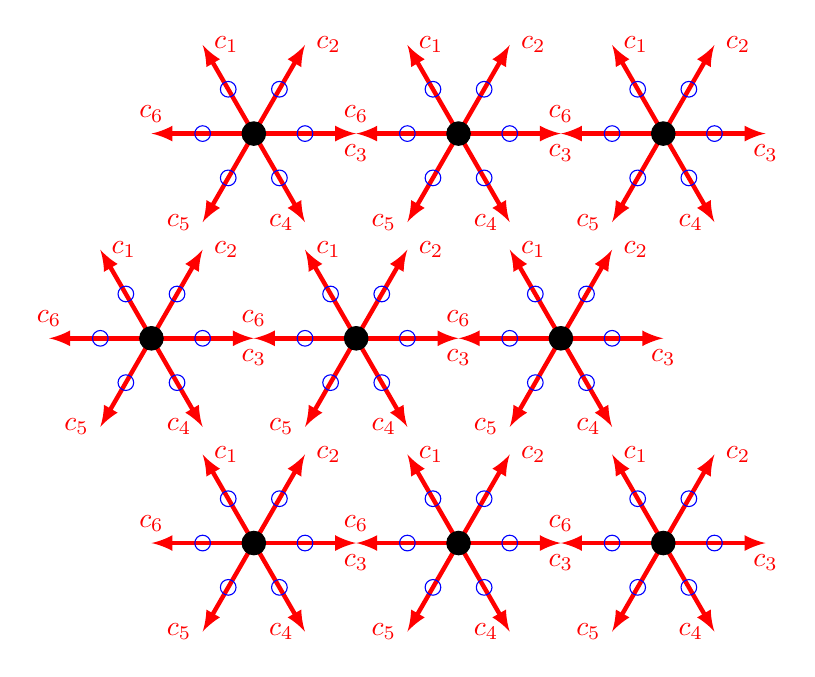
\begin{tikzpicture}[scale=0.65]
  \foreach \x in {0,4,8}
	{
	\foreach \y in {0,4,8}
		{
		\ifthenelse{\y = 4 }{
    \coordinate (Origin) at (0 + \x - 2,0 + \y);
    \coordinate (site1) at ({2 * cos(120) + \x- 2 }, {2 * sin(120) + \y });
    \coordinate (site2) at ({2 * cos(60) + \x - 2}, {2 * sin(60) + \y });
    \coordinate (site3) at ({2 * cos(0) + \x - 2}, {2 * sin(0) + \y });
    \coordinate (site4) at ({2 * cos(-60) + \x - 2}, {2 * sin(-60) + \y });
    \coordinate (site5) at ({2 * cos(-120) + \x - 2}, {2 * sin(-120) + \y });
    \coordinate (site6) at ({2 * cos(-180) + \x- 2 }, {2 * sin(-180) + \y });
    
	\draw [ultra thick,-latex,red] (Origin)
        -- (site1) node [right] {$c_1$};
    \draw [ultra thick,-latex,red] (Origin)
        -- (site2) node [right] {$c_2$};
    \draw [ultra thick,-latex,red] (Origin)
        -- (site3) node [below] {$c_3$};
    \draw [ultra thick,-latex,red] (Origin)
        -- (site4) node [left] {$c_4$};
    \draw [ultra thick,-latex,red] (Origin)
        -- (site5) node [left] {$c_5$};
    \draw [ultra thick,-latex,red] (Origin)
        -- (site6) node [above] {$c_6$};    
 	\coordinate (Origin) at (0 + \x- 2,0 + \y);
    \coordinate (site1) at ({cos(120) + \x- 2 }, { sin(120) + \y });
    \coordinate (site2) at ({ cos(60) + \x - 2}, { sin(60) + \y });
    \coordinate (site3) at ({ cos(0) + \x- 2 }, { sin(0) + \y });
    \coordinate (site4) at ({ cos(-60) + \x - 2}, { sin(-60) + \y });
    \coordinate (site5) at ({ cos(-120) + \x - 2}, { sin(-120) + \y });
    \coordinate (site6) at ({ cos(-180) + \x- 2 }, { sin(-180) + \y });
       
    \node[draw,circle,inner sep=3pt,fill] at (Origin) {};
    \node[draw,circle,inner sep=2pt,blue] at (site1) {};
    \node[draw,circle,inner sep=2pt,blue] at (site2) {};
    \node[draw,circle,inner sep=2pt,blue] at (site3) {};
    \node[draw,circle,inner sep=2pt,blue] at (site4) {};
    \node[draw,circle,inner sep=2pt,blue] at (site5) {};
    \node[draw,circle,inner sep=2pt,blue] at (site6) {};
    }
    %else
    {
       \coordinate (Origin) at (0 + \x ,0 + \y);
    \coordinate (site1) at ({2 * cos(120) + \x }, {2 * sin(120) + \y });
    \coordinate (site2) at ({2 * cos(60) + \x }, {2 * sin(60) + \y });
    \coordinate (site3) at ({2 * cos(0) + \x }, {2 * sin(0) + \y });
    \coordinate (site4) at ({2 * cos(-60) + \x }, {2 * sin(-60) + \y });
    \coordinate (site5) at ({2 * cos(-120) + \x }, {2 * sin(-120) + \y });
    \coordinate (site6) at ({2 * cos(-180) + \x}, {2 * sin(-180) + \y });    
	\draw [ultra thick,-latex,red] (Origin)
        -- (site1) node [right] {$c_1$};
    \draw [ultra thick,-latex,red] (Origin)
        -- (site2) node [right] {$c_2$};
    \draw [ultra thick,-latex,red] (Origin)
        -- (site3) node [below] {$c_3$};
    \draw [ultra thick,-latex,red] (Origin)
        -- (site4) node [left] {$c_4$};
    \draw [ultra thick,-latex,red] (Origin)
        -- (site5) node [left] {$c_5$};
    \draw [ultra thick,-latex,red] (Origin)
        -- (site6) node [above] {$c_6$};    
 	\coordinate (Origin) at (0 + \x,0 + \y);
    \coordinate (site1) at ({cos(120) + \x }, { sin(120) + \y });
    \coordinate (site2) at ({ cos(60) + \x }, { sin(60) + \y });
    \coordinate (site3) at ({ cos(0) + \x}, { sin(0) + \y });
    \coordinate (site4) at ({ cos(-60) + \x }, { sin(-60) + \y });
    \coordinate (site5) at ({ cos(-120) + \x }, { sin(-120) + \y });
    \coordinate (site6) at ({ cos(-180) + \x }, { sin(-180) + \y });
       
    \node[draw,circle,inner sep=3pt,fill] at (Origin) {};
    \node[draw,circle,inner sep=2pt,blue] at (site1) {};
    \node[draw,circle,inner sep=2pt,blue] at (site2) {};
    \node[draw,circle,inner sep=2pt,blue] at (site3) {};
    \node[draw,circle,inner sep=2pt,blue] at (site4) {};
    \node[draw,circle,inner sep=2pt,blue] at (site5) {};
    \node[draw,circle,inner sep=2pt,blue] at (site6) {};
    }
    }
 }
  \end{tikzpicture}
  \caption{Here is an example of a single hexagonal cell with 6 velocity vectors and 6 empty sites.}
  \label{figure:Hsingle-cell}
\end{figure}
\end{document}